\chapter{Random Variables}\label{S:RandomVariable}
It can be be inconvenient to work with a set of outcomes $\Omega$ upon which arithmetic is not possible.  We are often measuring our outcomes with subsets of real numbers.  Some examples include:

\begin{table}[ht]
\begin{tabular}{c c} \hline
Experiment & Possible measured outcomes\\ \hline
Counting the number of typos up to now & $\Zz_+:=\{0,1,2,\ldots\} \subset \Rz$ \\
Length in centi-meters of some shells on New Brighton beach & $(0,+\infty) \subset \Rz$ \\
Waiting time in minutes for the next Orbiter bus to arrive & $\Rz_+:=[0,\infty) \subset \Rz$\\
Vertical displacement from current position of a pollen on water & $\Rz$ \\ \hline
\end{tabular}
\end{table}

\section{Basic Definitions}\label{S:RVBasicDefs}

To take advantage of our measurements over the real numbers, in terms of its  metric structure and arithmetic, we need to formally define this measurement process using the notion of a random variable.
\begin{definition}[Random Variable]\label{D:RV}
Let $(\Omega, \C{F},P)$ be some probability triple.  Then, a {\bf Random Variable (RV)}, say $X$, is a function from the sample space $\Omega$ to the set of real numbers $\Rz$ 
\[
X : \Omega \rightarrow \Rz
\]
such that for every $x \in \Rz$, the inverse image of the half-open real interval $(-\infty,x]$ is an element of the collection of events $\C{F}$, i.e.:
\[
\text{for every $x$} \in \Rz, \qquad X^{[-1]}(\ (-\infty,x] \ ) := \{\omega: X(\omega) \leq x\} \in \C{F} \ .
\]
{\scriptsize This definition can be summarised by the statement that a RV is an  $\C{F}$-measurable map.}
We assign probability to the RV $X$ as follows:
\begin{equation}\label{E:ProbOfRV}
\p(X \leq x)  = \p(\ X^{[-1]}(\ (-\infty,x] \ ) \ ) := \p( \ \{\omega: X(\omega) \leq x\} \ ) \ .
\end{equation}
\end{definition}

\begin{definition}[Distribution Function]\label{D:DF}
The {\bf Distribution Function (DF)} or {\bf Cumulative Distribution Function (CDF)} of any RV $X$, over a  probability triple $(\Omega, \C{F},P)$, denoted by $F$ is:
\begin{equation}\label{E:DF}
F(x) := \p(X \leq x) = \p( \ \{\omega: X(\omega) \leq x\} \ ), \qquad \text{for any }\quad x \in \Rz \ .
\end{equation}
Thus, $F(x)$ or simply $F$ is a non-decreasing, right continuous, $[0,1]$-valued function over $\Rz$.  When a RV $X$ has DF $F$ we write $X \sim F$.
\end{definition}

A special RV that often plays the role of `building-block' in Probability and Statistics is the indicator function of an event $A$ that tells us whether the event $A$ has occurred or not.  Recall that an event belongs to the collection of possible events $\C{F}$ for our experiment.
\begin{definition}[Indicator Function]
The {\bf Indicator Function} of an event $A$ denoted $\BB{1}_A$ is defined as follows:
\begin{equation}
\BB{1}_A(\omega) := 
\begin{cases}
1 & \qquad \text{if} \quad \omega \in A \\
0 & \qquad \text{if} \quad \omega \notin A
\end{cases}
\end{equation}
\end{definition}
\begin{figure}[htpb]
\caption{The Indicator function of event $A \in \C{F}$ is a RV $\BB{1}_A$ with DF $F$ \label{F:RVIndic}}
\centering   \makebox{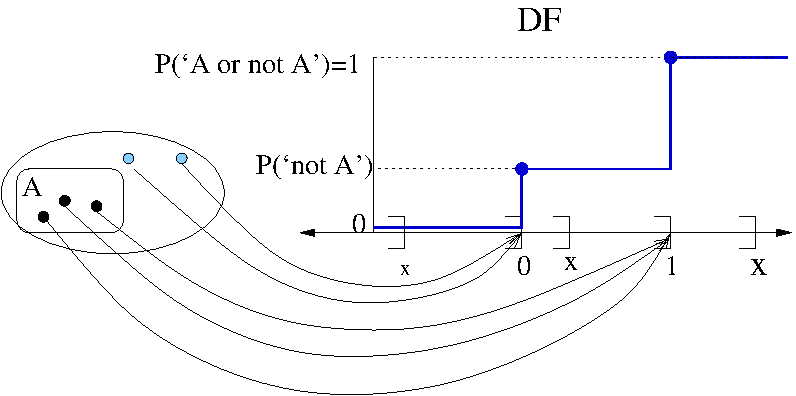
\includegraphics{figures/RVIndic}}
\end{figure}
\begin{classwork}[Indicator function is a random variable]
Let us convince ourselves that $\BB{1}_A$ is really a RV.  For $\BB{1}_A$ to be a RV, we need to verify that 
for any real number $x \in \Rz$, the inverse image $\BB{1}_A^{[-1]}( \ (- \infty, x] \ )$ is an event, ie :
\[
\BB{1}_A^{[-1]}( \ (- \infty, x] \ ) := \{\omega: \BB{1}_A(\omega) \leq x\} \in \C{F} \ .
\] 
All we can assume about the collection of events $\C{F}$ is that it contains the event $A$ and that it is a sigma algebra.  A careful look at the \hyperref[F:RVIndic]{Figure \ref*{F:RVIndic}} yields:
\begin{equation}
\BB{1}_A^{[-1]}( \ (- \infty, x] \ ) := \{\omega: \BB{1}_A(\omega) \leq x\} =
\begin{cases}
\emptyset & \text{if} \quad x < 0 \notag \\
A^c       & \text{if} \quad 0 \leq x < 1 \notag \\
A \cup A^c  = \Omega   & \text{if} \quad 1 \leq x  \notag 
\end{cases}
\end{equation}
Thus, $\BB{1}_A^{[-1]}( \ (- \infty, x] \ )$ is one of the following three sets that belong to $\C{F}$; (1) $\emptyset$, (2) $A^c$ and (3) $\Omega$ depending on the value taken by $x$ relative to the interval $[0,1]$.  We have proved that $\BB{1}_A$ is indeed a RV.
\end{classwork}
Some useful properties of the Indicator Function are:
\[
\BB{1}_{A^c} = 1 - \BB{1}_A, \qquad \BB{1}_{A \cap B} = \BB{1}_A \BB{1}_B, \qquad \BB{1}_{A \cup B} = \BB{1}_A + \BB{1}_B - \BB{1}_A \BB{1}_B
\]
We slightly abuse notation when $A$ is a single element set by ignoring the curly braces.
\begin{figure}[htpb]
\caption{A RV $X$ from a sample space $\Omega$ with $8$ elements to $\Rz$ and its DF $F$ \label{F:RVABC}}
\centering   \makebox{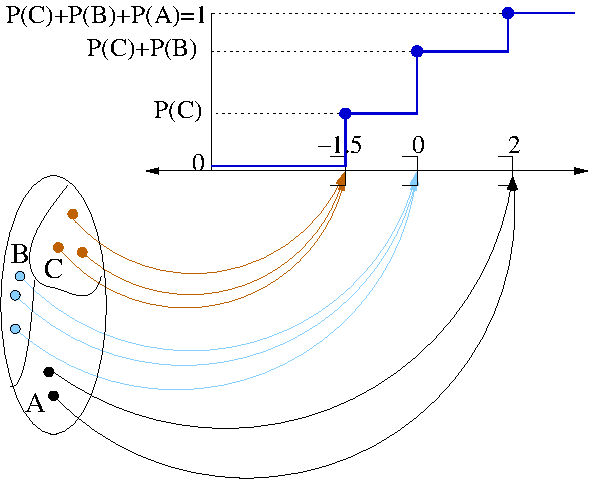
\includegraphics{figures/RV}}
\end{figure}
\begin{classwork}[A random variable with three values and eight sample points]
Consider the RV $X$ of \hyperref[F:RVABC]{Figure \ref*{F:RVABC}}.  Let the events $A = \{\omega_1, \omega_2\}$, $B = \{\omega_3, \omega_4, \omega_5\}$ and $C = \{\omega_6, \omega_7,\omega_8 \}$.  Define the RV $X$ formally.  What sets should $\C{F}$ minimally include?  What do you need to do to make sure that $\C{F}$ is a sigma algebra?
\vspace{4cm}
\end{classwork}

\section{An Elementary Discrete Random Variable}\label{S:ElemDiscRV}

When a RV takes at most countably many values from a discrete set $\Dz \subset \Rz$, we call it a {\bf discrete} RV.  Often, $\Dz$ is the set of integers $\Zz$.
\begin{definition}[probability mass function (PMF)]
Let $X$ be a discrete RV over a probability triple $(\Omega, \C{F},P)$.  We define the {\bf probability mass function} (PMF) $f$ of $X$ to be the function $f : \Dz \rightarrow [0,1]$ defined as follows:
\[
f(x) := \p(X=x) = \p( \ \{\omega: X(\omega) = x\} \ ), \qquad \text{where $x \in \Dz$.} 
\]
\end{definition}
The DF $F$ and PMF $f$ for a discrete RV $X$ satisfy the following:
\begin{enumerate}
\item  For any $x \in \Rz$,
\[
\p(X \leq x) = F(x) = \sum_{\Dz \ni y \leq x} f(y) := 
\sum_{y \ \in \  \Dz \cap (-\infty, x] } f(y) \ .
\]
\item For any $a,b \in \Dz$ with $a<b$,
\[
\p(a < X \leq b) = F(b) - F(a) = \sum_{y \ \in \  \Dz \cap (a, b] } f(y) \ .
\]
In particular, when $\Dz=\Zz$ and $a=b-1$,
\[
\p(b-1 < X \leq b) = F(b) - F(b-1) = f(b) = \p( \ \{ \omega : X(\omega) = b\} \ ) \ .
\]
\item And of course
\[
% \lim_{x \rightarrow \infty} F_X(x) = 1
\sum_{x \in \Dz} f(x) = 1
\]
\end{enumerate}

The Indicator Function $\BB{1}_A$ of the event that `$A$ occurs' for the $\theta$-specific experiment $\E{E}$ over some probability triple $(\Omega,\C{F},\p_{\theta})$, with $A \in \C{F}$, is the $\bernoulli(\theta)$ RV.  The parameter $\theta$ denotes the probability that `$A$ occurs' (see \hyperref[F:RVt1T]{Figure \ref*{F:RVt1T}} when $A$ is the event that `{\tt H} occurs').  This is our first example of a discrete RV.

\begin{model}[$\bernoulli(\theta)$]
Given a parameter $\theta \in [0,1]$, the probability mass function (PMF) for the $\bernoulli(\theta)$ RV $X$ is:
\begin{equation}\label{E:Bernoullipdf}
f(x;\theta)= \theta^x (1-\theta)^{1-x} \BB{1}_{\{0,1\}}(x) =
\begin{cases}
\theta & \text{if $x=1$,}\\
1-\theta & \text{if $x=0$,}\\
0 & \text{otherwise}
\end{cases}
\end{equation}
and its DF is:
\begin{equation}
F(x;\theta) =
\begin{cases}
1 & \text{if $1 \leq x$,}\\
1-\theta & \text{if $0 \leq x < 1$,}\\
0 & \text{otherwise}
\end{cases}
\end{equation}
We emphasise the dependence of the probabilities on the parameter $\theta$ by specifying it following the semicolon in the argument for $f$ and $F$ and by subscripting the probabilities, i.e.~$\p_{\theta}(X=1)=\theta$ and $\p_{\theta}(X=0)=1-\theta$.
\end{model}
\begin{figure}[htpb]
\caption{The Indicator Function $\BB{1}_{ \ {\tt H} \ }$ of the event `Heads occurs', for the experiment `Toss 1 times,' $\E{E}_{\theta}^{1}$, as the RV $X$ from the sample space $\Omega = \{ {\tt H}, {\tt T}\}$ to $\Rz$ and its DF $F$.  The probability that `Heads occurs' and that `Tails occurs' are $f(1;\theta)=\p_{\theta}(X=1) = \p_{\theta}({\tt H})=\theta$ and $f(0;\theta)=\p_{\theta}(X=0)=\p_{\theta}({\tt T})=1-\theta$, respectively.\label{F:RVt1T}}
\centering   \makebox{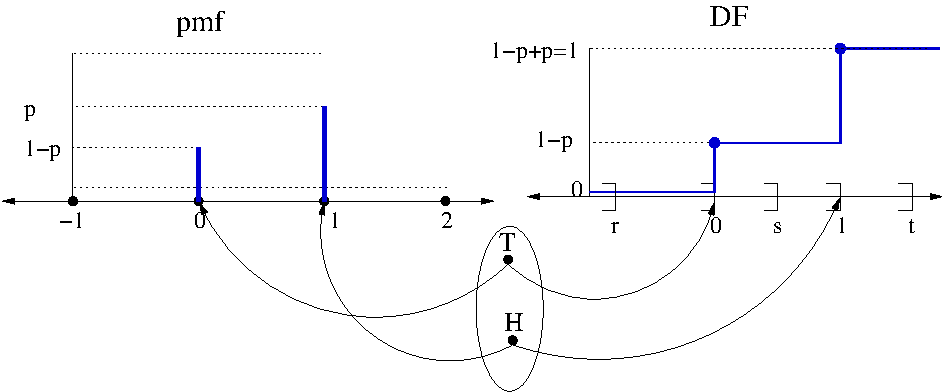
\includegraphics[width=6.5in]{figures/RVToss1}}
\end{figure}

\section{An Elementary Continuous Random Variable}\label{S:ElemContRV}

When a RV takes values in the continuum we call it a {\bf continuous} RV.  An example of such a RV is the vertical position (in micro meters) since the original release of a pollen grain on water.  Another example of a continuous RV is the volume of water (in cubic meters) that fell on the southern Alps last year.  
\begin{definition}[probability density function (PDF)]
A RV $X$ is said to be `continuous' if there exists a piecewise-continuous function $f$, called the probability density function (PDF) of $X$, such that for any $a, b \in \Rz$ with $a < b$,
\[
\p(a < X \leq b) = F(b)-F(a) = \int_a^b f(x) \ dx \ .
\]
\end{definition}
The following hold for a continuous RV $X$ with PDF $f$:
\begin{enumerate}
\item For any $x \in \Rz$, $\p(X=x)=0$.
\item Consequentially, for any $a,b \in \Rz$ with $a \leq b$,
\[
\p(a < X < b ) = \p(a < X \leq b) = \p(a \leq X \leq b) = \p(a \leq X < b) \ .
\]
\item By the fundamental theorem of calculus, except possibly at finitely many points (where the continuous pieces come together in the piecewise-continuous $f$):
\[
f(x) = \frac{d}{dx} F(x)
\]
\item And of course $f$ must satisfy:
\[
\int_{-\infty}^{\infty} f(x) \ dx = \p(-\infty < X < \infty) = 1 \ .
\] 
\end{enumerate}

An elementary and fundamental example of a continuous RV is the $\uniform(0,1)$ RV of \hyperref[M:Uniform01]{Model \ref*{M:Uniform01}}.  It forms the foundation for random variate generation and simulation.  In fact, it is appropriate to call this the fundamental model since every other experiment can be obtained from this one.

\begin{model}[The Fundamental Model]\label{M:Uniform01}
The probability density function (PDF) of the fundamental model or the $\uniform(0,1)$ RV is
\begin{equation}\label{E:Uniform01pdf}
f(x) = \BB{1}_{[0,1]}(x) = 
\begin{cases}
1 & \text{if $0 \leq x \leq 1$,}\\
0 & \text{otherwise}
\end{cases}
\end{equation}
and its distribution function (DF) or cumulative distribution function (CDF) is:
\begin{equation}\label{E:Uniform01DF}
F(x) := \int_{- \infty}^x f(y) \ dy =
\begin{cases}
0 & \text{if $x < 0$,} \\
x & \text{if $0 \leq x \leq 1$,}\\
1 & \text{if $x > 1$} 
\end{cases}
\end{equation}
Note that the DF is the identity map in $[0,1]$.  The PDF and DF are depicted in \hyperref[F:unif01]{Figure~\ref*{F:unif01}}.
\begin{figure}[htpb]
\caption{A plot of the PDF and DF or CDF of the $\uniform(0,1)$ continuous RV $X$.\label{F:unif01}}
\centering   \makebox{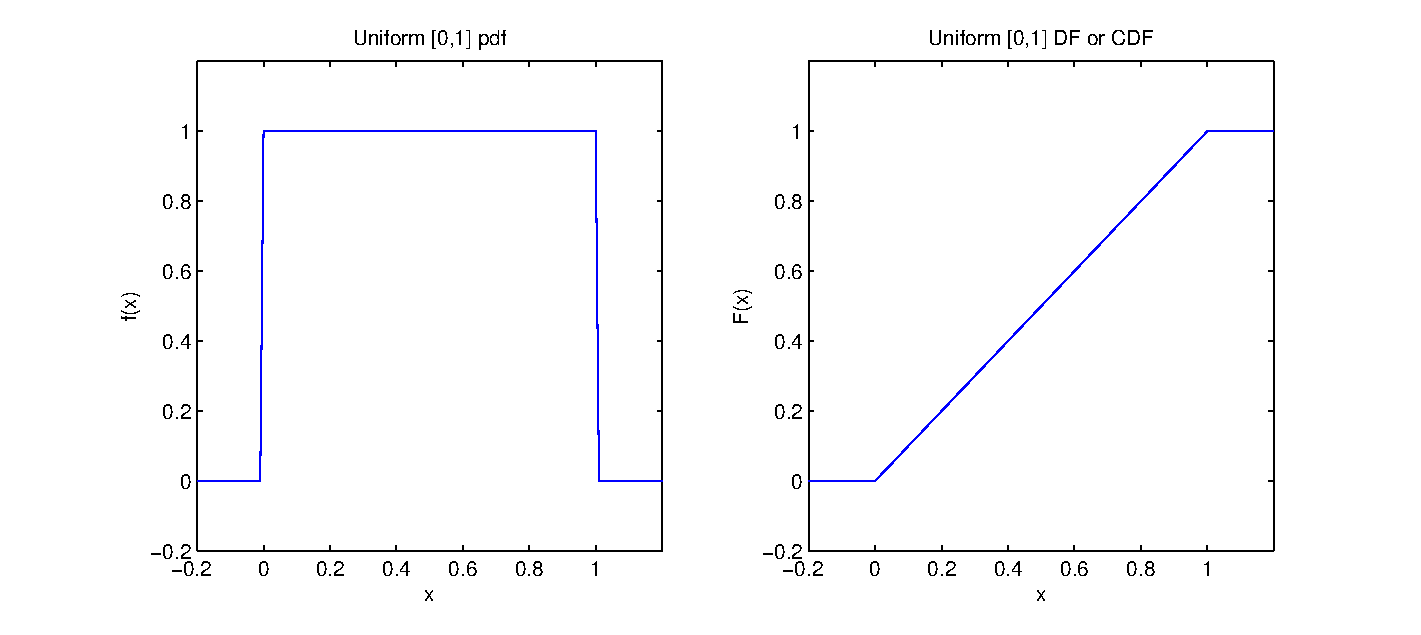
\includegraphics[width=6.5in]{figures/Unif01pdfcdf}}
\end{figure}
\end{model}

\remove{
\begin{labwork}[PDF of $\uniform(0,1)$ RV]\label{LW:Unif01Pdf}
Let us encode the PDF of $\uniform(0,1)$ as an M-file in {\sc Matlab}.  Notice that the PDF function assigns $1$ to every value of $x \in [0,1]$ and $0$ to every value of $x \notin [0,1]$.  So, the problem mostly boils down to finding the entries inside and outside the range.  We can use {\sc Matlab}'s built-in {\tt find} function for this purpose.  We give an example to illustrate the syntax of {\tt find}.
\begin{VrbM}
>> Xs=[0.2511    1.6160    0.4733    -5.3517    0.8308    0.5853    2.5497] % an array Xs with real values 
Xs =    0.2511    1.6160    0.4733   -5.3517    0.8308    0.5853    2.5497
\end{VrbM}
We can obtain the indices of {\tt Xs} whose values are $\geq 0$, i.e.~$\{i: {\tt Xs}(i) \geq 0 \}$ and the indices of {\tt Xs} whose values are $\leq 1$, i.e.~$\{i: {\tt Xs}(i) \leq 1 \}$ as follows:
\begin{VrbM}
>> find(Xs >= 0)
ans =     1     2     3     5     6     7
>> find(Xs <= 1)
ans =     1     3     4     5     6
\end{VrbM}
The intersection of the two sets of indices, i.e.~$\{i: {\tt Xs}(i) \geq 0 \ \text{ and } \  {\tt Xs}(i) \leq 1 \} = \{i: 0 \leq {\tt Xs}(i) \leq 1 \}$ can be obtained by {\tt \&}, the Boolean and, as follows:
\begin{VrbM}
>> find(Xs >= 0 & Xs <= 1)
ans =     1     3     5     6
\end{VrbM}
Finally, we know which indices of the {\tt Xs} array should have the PDF value of $1$.  The remaining indices of {\tt Xs} should therefore have the PDF value of $0$.  Let us declare an array called {\tt Pdf} for the PDF values corresponding to the {\tt Xs}.  We can initialise this array with zeros using the {\tt zeros} function and make it of the same size as {\tt Xs} as follows:
\begin{VrbM}
>> size(Xs)
ans =     1     7
>> Pdf = zeros(1,7)
Pdf =     0     0     0     0     0     0     0
\end{VrbM}
Now, we can set the indices $1,3,5,6$ (returned by {\tt find(Xs >= 0 \& Xs <= 1)}) of {\tt Pdf} array to 1.
\begin{VrbM}
>> Pdf([1     3     5     6])=1
Pdf =     1     0     1     0     1     1     0
\end{VrbM}
We can modularise this process for an arbitrary input array {\tt x} via a function in the following M-file.
\VrbMf[label=Unif01Pdf.m]{scripts/Unif01Pdf.m} 
Let us call the function we wrote called {\tt Unif01Pdf} next.
\begin{VrbM}
>> help Unif01Pdf
  Unif01Pdf(x) returns the PDF of Uniform(0,1) RV X
  the input x can be an array
>> Xs
Xs =    0.2511    1.6160    0.4733   -5.3517    0.8308    0.5853    2.5497
>> Unif01Pdf(Xs)
ans =     1     0     1     0     1     1     0
\end{VrbM}
\end{labwork}

\begin{labwork}[CDF of $\uniform(0,1)$ RV]\label{LW:Unif01Cdf}
Understand each step in the function {\tt Unif01Cdf}:
\VrbMf[label=Unif01Cdf.m]{scripts/Unif01Cdf.m} 
When we type in {\tt help Unif01Cdf}, {\tt Xs} and {\tt Unif01Cdf(Xs)} we can confirm that the {\tt Unif01Cdf} function is correctly reporting the CDF values of the input array {\tt Xs}.
\begin{VrbM}
>> help Unif01Cdf
  Unif01Cdf(x) returns the CDF of Uniform(0,1) RV X
  the input x can be an array 
>> Xs
Xs =    0.2511    1.6160    0.4733   -5.3517    0.8308    0.5853    2.5497
>> Unif01Cdf(Xs)
ans =    0.2511    1.0000    0.4733         0    0.8308    0.5853    1.0000
\end{VrbM}
\end{labwork}

\begin{labwork}[Plot of the PDF and the CDF for the $\uniform(0,1)$ RV]\label{LW:PlotUnif01PdfCdf}
Generate the plot of the PDF and the CDF for the $\uniform(0,1)$ RV $X$ by following the commands below.  Go through every step and understand each command when you reproduce the plot.
\VrbMf[label=plotunif.m]{scripts/plotunif.m} 
The plot was saved as an encapsulated postscript file from the File menu of the Figure window and is displayed in \hyperref[F:unif01]{Figure~\ref*{F:unif01}}.
 \end{labwork}
}

{\bf **tossing a fair coin infinitely often and the fundamental model}

%TODO\input{figures/UnifsInUnif.tex}

--- The fundamental model is equivalent to infinite tosses of a fair coin (see using binary expansion of any $x \in (0,1)$)

--- The fundamental model has infinitely many copies of itself within it!


{\bf **universality of the fundamental model}

--- one can obtain any other random object from the fundamental model!
\newpage


\section{Expectations}\label{S:Expectations}
It is convenient to summarise a RV by a single number.  This single number can be made to represent some average or expected feature of the RV via an integral with respect to the density of the RV.  

\begin{definition}[Expectation of a RV]
The {\bf expectation}, or {\bf expected value}, or {\bf mean}, or {\bf first moment}, of a random variable $X$, with distribution function $F$ and density $f$, is defined to be
\begin{equation}\label{E:Mean}
\e(X) := \int x\,dF(x) = 
\begin{cases}
\sum_x x f(x) & \qquad \text{if $X$ is discrete} \\
\int x f(x)\,dx  & \qquad \text{if $X$ is continuous} \  ,
\end{cases}
\end{equation}
provided the sum or integral is well-defined.  We say the expectation exists if
\begin{equation}\label{E:ExpectationExists}
\int \left|x\right|\,dF(x) < \infty \ .
\end{equation}
Sometimes, we denote $\e(X)$ by $\e X$ for brevity.  Thus, the expectation is a single-number summary of the RV $X$ and may be thought of  as the average.
We subscript $E$ to specify the parameter $\theta \in \BB{\Theta}$ with respect to which the integration is undertaken. 
\[
\e_{\theta} X := \int x\,dF(x;\theta)
\]
\end{definition}

\begin{definition}[Variance of a RV]\label{D:VarianceofX}
Let $X$ be a RV with mean or expectation $\e(X)$.  Variance of $X$ denoted by $\V(X)$ or $VX$ is
\[
\V(X) := \e \left((X-\e(X))^2\right) = \int (x-\e(X))^2 \,d F(x) \ ,
\]
provided this expectation exists.  The {\bf standard deviation} denoted by $\sd(X) := \sqrt{\V(X)}$.
Thus variance is a measure of ``spread'' of a distribution.
\end{definition}

\begin{definition}[$k$-th moment of a RV]
We call 
\[
\e(X^k) = \int x^k\,dF(x)
\]
as the $k$-th moment of the RV $X$ and say that the $k$-th moment exists when $\e(|X|^k) < \infty$.  We call the following expectation as the $k$-th central moment:
\[
\e \left((X- \e(X))^k\right) \ .
\]
\end{definition}

\subsection*{Properties of Expectations}

\begin{enumerate}
\item If the $k$-th moment exists and if $j<k$ then the $j$-th moment exists.

\item If $X_1,X_2,\ldots,X_n$ are RVs and $a_1,a_2,\ldots,a_n$ are constants, then 
\begin{equation}\label{E:EofLinCombofRVs}
\e \left( \sum_{i=1}^n a_i X_i \right) = \sum_{i=1}^n a_i \e(X_i) \ .
\end{equation}
\item Let $X_1,X_2,\ldots,X_n$ be independent RVs, then
\begin{equation}\label{E:EofProdIndRVs}
\e \left(  \prod_{i=1}^n X_i \right) = \prod_{i=1}^{n} \e(X_i) \ .
\end{equation}
\item $\V(X) = \e(X^2) - (\e(X))^2$ \ . [prove by completing the square and applying \eqref{E:EofLinCombofRVs}]
\item If $a$ and $b$ are constants then:
\begin{equation}\label{E:VofAffineofRVs}
\V(aX+b) = a^2\V(X) \ . 
\end{equation}
\item If $X_1,X_2,\ldots,X_n$ are independent and $a_1,a_2,\ldots,a_n$ are constants, then:
\begin{equation}\label{E:VofLinCombofRVs}
\V \left(  \sum_{i=1}^n a_i X_i \right) = \sum_{i=1}^n a_i^2 \V(X_i) \ .
\end{equation}
\end{enumerate}

\paragraph{Mean and variance of $\bernoulli(\theta)$ RV:}
Let $X \sim \bernoulli(\theta)$.  Then, 
\[
\e(X) = \sum_{x=0}^1 x f(x) = (0 \times (1-\theta)) + (1 \times \theta) = 0+\theta=\theta \ ,
\]
\[
\e(X^2) =  \sum_{x=0}^1 x^2 f(x) =  (0^2 \times (1-\theta) ) + (1^2 \times \theta) = 0+\theta= \theta \ ,
\]
\[
\V(X) = \e(X^2) - (\e(X))^2 = \theta - \theta^2 = \theta(1-\theta) \ .
\]
Parameter specifically,
\[
\e_{\theta}(X)=\theta \qquad \text{and} \qquad \V_{\theta}(X)=\theta(1-\theta) \ .
\]
\begin{figure}[htpb]
\caption{Mean ($\e_{\theta}(X)$), variance ($\V_{\theta}(X)$) and the rate of change of variance ($\frac{d}{d \theta} \V_{\theta}(X)$) of a $\bernoulli(\theta)$ RV $X$ as a function of the parameter $\theta$.\label{F:MeanVarBernoulli}}
\centering   \makebox{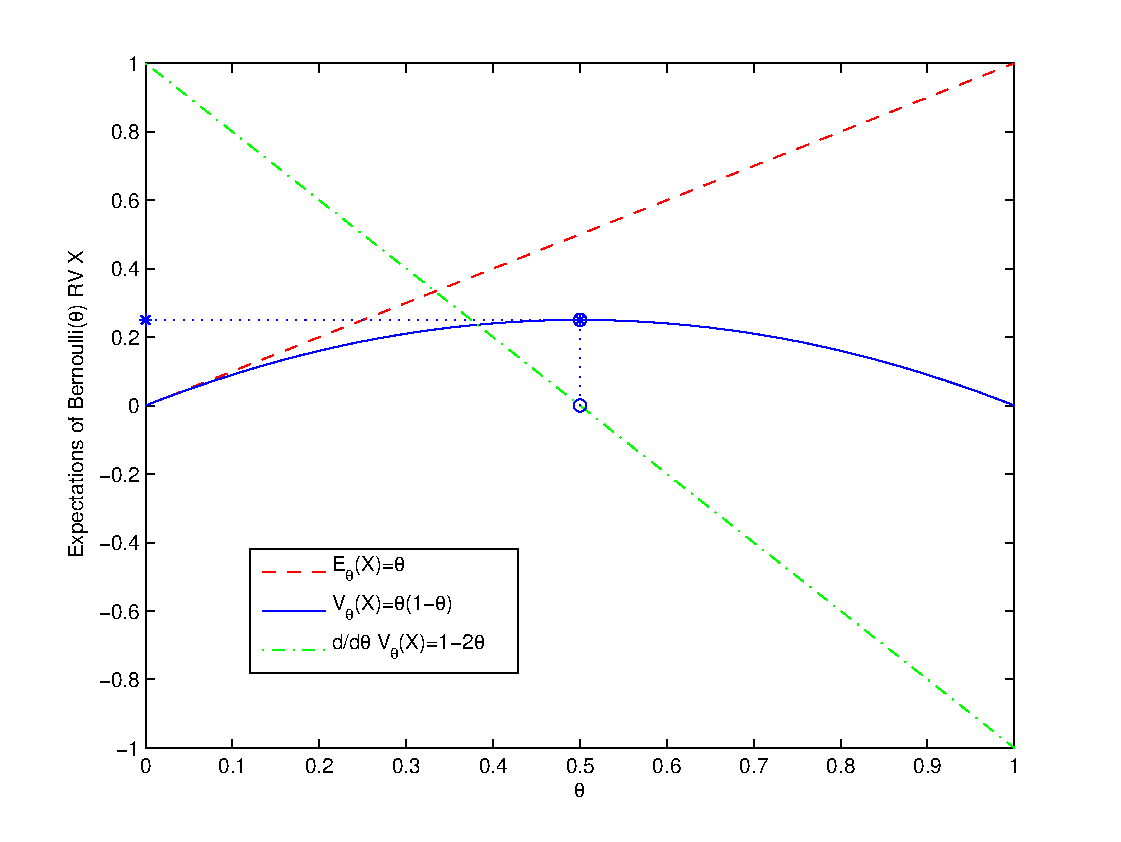
\includegraphics[width=5.0in]{figures/PlotMeanVarBernoulli}}
\end{figure}

Maximum of the variance $\V_{\theta}(X)$ is found by setting the derivative to zero, solving for $\theta$ and showing the second derivative is locally negative, i.e.~$\V_{\theta}(X)$ is concave down:
\[
\V_{\theta}'(X) := \frac{d}{d \theta} \V_{\theta}(X) = 1-2 \theta = 0  \iff \theta = \frac{1}{2} \ , 
\qquad \V_{\theta}''(X) := \frac{d}{d \theta} \left( \frac{d}{d \theta} \V_{\theta}(X) \right) = -2 < 0 \ ,
\]
\[
\max_{\theta \in [0,1]} \V_{\theta}(X) = \frac{1}{2} \left(1-\frac{1}{2} \right) = \frac{1}{4} \ , 
\text{since $\V_{\theta}(X)$ is maximized at $\theta = \frac{1}{2}$}
\]
The plot depicting these expectations as well as the rate of change of the variance are depicted in \hyperref[F:MeanVarBernoulli]{Figure \ref*{F:MeanVarBernoulli}}.  Note from this Figure that $\V_{\theta}(X)$ attains its maximum  value of $1/4$ at $\theta=0.5$ where $\frac{d}{d\theta}\V_{\theta}(X)=0$.  Furthermore, we know that we don't have a minimum at $\theta=0.5$ since the second derivative $\V_{\theta}''(X) = -2$ is negative for any $\theta \in [0,1]$.  This confirms that $\V_{\theta}(X)$ is concave down and therefore we have a maximum of $\V_{\theta}(X)$ at $\theta=0.5$.  We will revisit this example when we employ a numerical approach called Newton-Raphson method to solve for the maximum of a differentiable function by setting its derivative equal to zero.

\paragraph{Mean and variance of $\uniform(0,1)$ RV:}
Let $X \sim \uniform(0,1)$.  Then, 
\[
\e(X) = \int_{x=0}^1 x f(x)\, dx = \int_{x=0}^1 x \ 1 \, dx = \frac{1}{2} \left( x^2 \right]_{x=0}^{x=1} = \frac{1}{2} \left( 1-0 \right) = \frac{1}{2} \ ,
\]
\[
\e(X^2) = \int_{x=0}^1 x^2 f(x)\, dx = \int_{x=0}^1 x^2 \ 1 \, dx =  \frac{1}{3} \left( x^3 \right]_{x=0}^{x=1} = \frac{1}{3} \left( 1-0 \right) = \frac{1}{3} \ ,
\]
\[
\V(X) = \e(X^2) - (\e(X))^2 = \frac{1}{3}  - \left( \frac{1}{2} \right)^2  = \frac{1}{3}  - \frac{1}{4} = \frac{1}{12} \ .
\]

\begin{prop}[Winnings on Average]
Let $Y = r(X)$.  Then
\[
\e(Y) = \e(r(X)) = \int r(x)\, d F(x) \ .
\]
Think of playing a game where we draw $x \sim X$ and then I pay you $y=r(x)$.  Then your average income is $r(x)$ times the chance that $X=x$, summed (or integrated) over all values of $x$.
\end{prop}

\begin{example}[Probability is an Expectation]
Let $A$ be an event and let $r(X)=\BB{1}_{A}(x)$.  Recall $\BB{1}_A(x)$ is $1$ if $x \in A$ and $\BB{1}_A(x)=0$ if $x \notin A$.  Then
\begin{equation}\label{E:ExpectationofIndicator}
\e(\BB{1}_A(X)) = \int \BB{1}_A(x)\, dF(x) = \int_A f(x)\, dx = \p(X \in A) = \p(A)
\end{equation}
Thus, probability is a special case of expectation.  Recall our LTRF motivation for the definition of probability and make the connection.
\end{example}
%\begin{example}[Exponential of the $Uniform(0,1)$ RV]
%Let $X \sim Uniform(0,1)$.  Let $Y=r(x)=e^X$.  Then,
%\[
%\e(Y) = \int_0^1 e^x f(x) dx = \int_0^1 e^x 1 \ dx = e-1 \ .
%\]
%You could have also found out that the density $f(y)=1/y$ for the RV $Y$, provided $1<y<e$, and $0$ otherwise.  Again,
%\[
%\e(Y) = \int_1^e y f(y) dy = \int_1^e y \frac{1}{y} dy = \int_1^e 1 \ dy = e-1 \ .
%\]
%\end{example}

\section{Stochastic Processes}\label{S:StochProc}
\begin{definition}[Independence of RVs]\label{D:IndRVs}
A finite or infinite sequence of RVs $X_1,X_2,\ldots$ is said to be independent or independently distributed if
\[
\p(X_{i_1} \leq x_{i_1}, X_{i_2} \leq x_{i_2}, \ldots,  X_{i_k} \leq x_{i_k} ) = \p(X_{i_1} \leq x_{i_1}) \p(X_{i_2} \leq x_{i_2}) \cdots,  \p(X_{i_k} \leq x_{i_k} )
\]
for any distinct subset $\{i_1,i_2,\ldots,i_l\}$ of indices of the sequence of RVs and any sequence of real numbers $x_{i_1},x_{i_2},\ldots,x_{i_k}$.

By the above definition, the sequence of {\bf discrete} RVs $X_1,X_2,\ldots$ taking values in an at most countable set $\Dz$ are said to be independently distributed if for any distinct subset of indices $\{i_1,i_2,\ldots,i_k\}$ such that the corresponding RVs $X_{i_1},X_{i_2},\ldots,X_{i_k}$ exists as a distinct subset of our original sequence of RVs $X_1,X_2,\ldots$ and for any elements $x_{i_1}, x_{i_2},\ldots,x_{i_k}$ in $\Dz$, the following equality is satisfied:
\[
\p(X_{i_1}= x_{i_1}, X_{i_2} = x_{i_2}, \ldots,  X_{i_k} = x_{i_k} ) = \p(X_{i_1} = x_{i_1}) \p(X_{i_2} = x_{i_2}) \cdots  \p(X_{i_k} = x_{i_k})
\]
\end{definition}
For an independent sequence of RVs $\{X_1,X_2,\ldots\}$, we have
\begin{eqnarray}
&&\p(X_{i+1} \leq x_{i+1} | X_{i} \leq x_{i}, X_{i-1} \leq x_{i-1}, \ldots, X_1 \leq x_1) \notag\\
\notag \\
&=& \frac{\p(X_{i+1} \leq x_{i+1}, X_{i} \leq x_{i}, X_{i-1} \leq x_{i-1}, \ldots, X_1 \leq x_1)}{\p(X_{i} \leq x_{i}, X_{i-1} \leq x_{i-1}, \ldots, X_1 \leq x_1)} \notag \\
\notag \\
&=& \frac{\p(X_{i+1} \leq x_{i+1}) \p(X_{i} \leq x_{i}) \p(X_{i-1} \leq x_{i-1}) \cdots \p(X_1 \leq x_1)}{\p(X_{i} \leq x_{i}) \p(X_{i-1} \leq x_{i-1}) \cdots \p(X_1 \leq x_1)} \notag \\
\notag \\
&=& \p(X_{i+1} \leq x_{i+1}) \notag 
\end{eqnarray}
The above equality that 
\[
\p(X_{i+1} \leq x_{i+1} | X_{i} \leq x_{i}, X_{i-1} \leq x_{i-1}, \ldots, X_1 \leq x_1) =  \p(X_{i+1} \leq x_{i+1}) 
\]
simply says that the conditional distribution of the RV $X_{i+1}$ given all previous RVs $X_i,X_{i-1},\ldots,X_1$ is simply determined by the distribution of $X_{i+1}$.

When a sequence of RVs are not independent they are said to be {\bf dependent}.  

\begin{definition}[Stochastic Process]
A collection of RVs  \[
\left(X_{\alpha} \right)_{\alpha \in N} := \left( \  X_{\alpha} : \alpha \in \Az \  \right)
\]
is called a {\bf stochastic process}.  Thus, for every $\alpha \in  \Az$, the index set of the stochastic process, $X_{\alpha}$ is a RV.  If the index set $ \Az  \subset \Zz$ then we have  a {\bf discrete time stochastic process}, typically denoted by 
\[
\left(X_i\right)_{i \in \Zz} := \ldots, X_{-2},X_{-1},X_0, X_1,X_2,\ldots , \  \text{or}
\]
\[
\left( X_i \right)_{i \in \Nz} := X_1,X_2,\ldots , \  \text{or}
\]
\[
\left( X_i \right)_{i \in [n]} := X_1,X_2,\ldots , X_n , \ \text{where, } [n]:= \{1,2,\ldots,n\} \ .
\]
If $\Az \subset \Rz$ then we have a {\bf continuous time stochastic process}, typically denoted by $\{X_t\}_{t \in \Rz}$, etc.  
\end{definition}

\begin{definition}[Independent and Identically Distributed (IID)]
The finite or infinite sequence of RVs or the stochastic process $X_1, X_2,\ldots$ is said to be independent and identically distributed or IID if :
\begin{itemize}
\item they are an idependently distributed according to \hyperref[D:IndRVs]{Definition \ref*{D:IndRVs}}, and
\item $F(X_1) = F(X_2) = \cdots $, ie.~all the $X_i$'s have the same DF $F(X_1)$.
\end{itemize}
This is perhaps the most elementary class of stochastic processes and we succinctly denote it by
\[
\left(X_i\right)_{i \in [n]} := X_1, X_2,\ldots, X_n \overset{\IID}{\sim} F, \quad \text{or} \quad \left(X_i\right)_{i \in \Nz} := X_1, X_2,\ldots  \overset{\IID}{\sim} F \ .
\]
We sometimes replace the DF $F$ above by the name of the RV.
 \end{definition}
 
\begin{definition}[Independently Distributed]
The sequence of RVs or the stochastic process $\left(X_i\right)_{i \in \Nz} := X_1, X_2,\ldots$ is said to be independently distributed if :
\begin{itemize}
\item $X_1, X_2,\ldots$ is independently distributed according to \hyperref[D:IndRVs]{Definition \ref*{D:IndRVs}}.
\end{itemize}
This is a class of stochastic processes that is more general than the IID class.
\end{definition}

\remove{
Let us consider a few discrete RVs for the simple coin tossing experiment $\E{E}_{\theta}^{3}$ that build on the $\bernoulli(\theta)$ RV $X_i$ for the $i$-th toss in an {\bf independent and identically distibuted (IID.)} manner.
\begin{table}[htpb]
\caption{The $8$ $\omega$'s in the sample space $\Omega$ of the experiment $\E{E}_{\theta}^{3}$ are given in the first row above.  The RV $Y$ is the number of `Heads' in the $3$ tosses and the RV $Z$ is the number of `Tails' in the $3$ tosses.  Finally, the RVs $Y'$ and $Z'$ are the indicator functions of the event that `all three tosses were Heads' and the event that `all three tosses were Tails', respectively.\label{T:T3XRVs}}
 \begin{tabular}{r c c c c c c c c l}
 \hline
$\omega$:    & {\tt HHH} & {\tt HHT} & {\tt HTH} & {\tt HTT} & {\tt THH} & {\tt THT} & {\tt TTH} & {\tt TTT} & RV Definitions / Model \\ \hline
 \\
$\p(\omega)$: & $\frac{1}{8}$ & $\frac{1}{8}$ & $\frac{1}{8}$ & $\frac{1}{8}$ &  $\frac{1}{8}$ & $\frac{1}{8}$ & $\frac{1}{8}$ & $\frac{1}{8}$  & $X_i \overset{\IID}{\sim} \bernoulli(\frac{1}{2})$ \\
 \\
$Y(\omega)$: & 3         & 2         & 2         & 1         & 2         & 1         & 1         & 0        & $Y := X_1+X_2+X_3$ \\
 \\
$Z(\omega)$: & 0         & 1         & 1         & 2         & 1         & 2         & 2         & 3        & $Z := (1-X_1)+(1-X_2)+(1-X_3)$ \\
 \\
$Y'(\omega)$: & 1         & 0         & 0         & 0         & 0         & 0         & 0         & 0       & $Y' :=  X_1 X_2 X_3$ \\
\\
$Z'(\omega)$: & 0         & 0         & 0         & 0         & 0         & 0         & 0         & 1       & $Y' :=  (1-X_1)(1-X_2)(1-X_3)$ \\ \hline
 \end{tabular}
 \end{table}
 \begin{classwork}[Two random variables of `toss a coin thrice' experiment]
Describe the probability of the RV $Y$ and $Y'$ of \hyperref[T:T3XRVs]{Table \ref*{T:T3XRVs}} in terms of its PMF.  Repeat the process for the RV $Z$ in your spare time.
 \begin{eqnarray}
 \p(Y=y) =%:= \p(\{\omega: Y(\omega)=y\}) = 
 \begin{cases}
 \qquad & \qquad \notag \\
 \qquad & \qquad \notag \\
 \qquad & \qquad \notag \\
 \qquad & \qquad \notag
 \end{cases} 
 & \qquad \qquad \qquad \qquad \qquad
\p(Y'=y') =%:= \p(\{\omega: Y'(\omega)=y'\}) = 
 \begin{cases}
 \qquad & \qquad \notag \\
 \qquad & \qquad \notag 
 \end{cases}
 \end{eqnarray}
 \end{classwork}
 
 \begin{classwork}[The number of `Heads' given there is at least one `Tails']
 Consider the following two questions.
 \begin{enumerate}
\item What is conditional probability $\p(Y|Y'=0)$ ?
%{\color{Gray}{
 \[
 \begin{array}{c c c c}
 \hline \\
 \p(Y=y | Y'=0) & =\frac{\p(Y=y,Y'=0)}{\p(Y'=0)} & =\frac{\p(\{\omega: Y(\omega)=y \  \cap \ Y'(\omega)=0\})}{\p(\{\omega: Y'(\omega)=0\})} & = ? \\ \hline \\
 \\
 \p(Y=0 | Y'=0) & \frac{\p(Y=0,Y'=0)}{\p(Y'=0)} & \frac{\frac{1}{8}}{\frac{1}{8}+\frac{1}{8}+\frac{1}{8}+\frac{1}{8}+\frac{1}{8}+\frac{1}{8}+\frac{1}{8}} & \frac{1}{7} \\
\\
\p(Y=1 | Y'=0) & \frac{\p(Y=1,Y'=0)}{\p(Y'=0)} & \frac{\frac{1}{8}+\frac{1}{8}+\frac{1}{8}}{\frac{1}{8}+\frac{1}{8}+\frac{1}{8}+\frac{1}{8}+\frac{1}{8}+\frac{1}{8}+\frac{1}{8}} & \frac{3}{7} \\
\\
\p(Y=2 | Y'=0) & \frac{\p(Y=2,Y'=0)}{\p(Y'=0)} & \frac{\frac{1}{8}+\frac{1}{8}+\frac{1}{8}}{\frac{1}{8}+\frac{1}{8}+\frac{1}{8}+\frac{1}{8}+\frac{1}{8}+\frac{1}{8}+\frac{1}{8}} & \frac{3}{7} \\
\\
\p(Y=3 | Y'=0) & \frac{\p(Y=3,Y'=0)}{\p(Y'=0)} & \frac{\p(\emptyset)}{\frac{1}{8}+\frac{1}{8}+\frac{1}{8}+\frac{1}{8}+\frac{1}{8}+\frac{1}{8}+\frac{1}{8}} & 0 \\
\\ \hline
\p(Y \in \{0,1,2,3\} | Y'=0) & \frac{\sum_{y=0}^3{\p(Y=y,Y'=0)}}{\p(Y'=0)} & \frac {\frac{1}{8}+\frac{1}{8}+\frac{1}{8}+\frac{1}{8}+\frac{1}{8}+\frac{1}{8}+\frac{1}{8}}{\frac{1}{8}+\frac{1}{8}+\frac{1}{8}+\frac{1}{8}+\frac{1}{8}+\frac{1}{8}+\frac{1}{8}} & 1 \\ \hline
 \end{array}
 \]
% }}
\item What is $\p(Y|Y'=1)$ ?
%{\color{Gray}{
 \[
\p(Y=y | Y'=1) = 
\begin{cases}
1 & \text{if $y=3$} \\
0 & \text{otherwise}
 \end{cases}
 \]
 %}}
 \end{enumerate}
 \end{classwork}

}
